\section{Droplet deformation in stokestain dilute emulsions}




We now consider a dilute mono-disperse suspension of spherical droplet of radius $a$ without mass transfer. 
The dispersed  and continuous phases are considered Newtonian fluids defined by the constant viscosities $\mu_k$ and density $\rho_k$.
Additionally, the surface tension coefficient at the interface between both fluids is noted $\gamma$. 
Because we consider a small droplet Reynolds number, we assert that only the averaged mass and momentum equations are sufficient to describe the mixture. 
% In most of the industrial applications however, surfactants or/and non-uniform temperature gradient are present in the emulsion, both of which influence the value of the surface tension coefficient at the interface of the droplets.
% Hence, in this study we consider a non-uniform surface tension distribution at the interface of the droplets. 
\begin{table}
    \centering
    \begin{tabular}{|c|ccl|}\hline
    & Conservation law & mass & momentum \\ \hline
    Conserved quantity & $f_k^0$  & $\rho_k$ & $\rho_k \textbf{u}_k^0$ \\
    Source term & $s_k^0$  & $0$ & $\rho_k \textbf{g}$ \\
    Diffusive flux & $\Phi_k^0$ & 0 & $\bm\sigma_k^0 = -p_k^0 + \mu_k (\grad \textbf{u}_k^0 + \grad \textbf{u}_k^0)$ \\
    Surface diffusive flux & $\Phi_\Gamma^0$ & 0 & $\bm\sigma_\Gamma^0 = \gamma (\bm\delta - \textbf{nn})$ \\\hline
    \end{tabular}
    \begin{tabular}{|c|c|}\hline\hline
    Velocity scale & $U = \mathcal{O}(|\textbf{u}_f|)$ or $\mathcal{O}(|\textbf{u}_f - \textbf{u}_p|)$ \\
    Macroscopic length scale & $L$ \\
    Droplets radius & $a$ \\
    Viscosity ratio & $\lambda = \mu_d / \mu_f$ \\
    Density ratio & $\zeta = \rho_d / \rho_f$ \\
    Reynolds number & $Re = \rho_f a U / \mu_f$   \\
    Capillary number & $Ca = \mu_f U / \gamma$ \\\hline
    \end{tabular}
    \caption{Definition of the physical quantities and local constitutive laws for phase $\rho_k$, and dimensionless numbers of the closure problem.}
    \label{tab:qte_Newtonian}
\end{table}
The physical quantities to be conserved as well as the dimensionless number of the problem are summaries \ref{tab:qte_Newtonian}. 

After presenting in details the momentum equations for mono-disperse suspension of droplets, we dive into the closure problem. 
In the averaged equation we neglect the droplet inertia, thus all the terms of $\mathcal{O}(Re \phi)$ are not considered.
Moreover, we will consider spherical droplets, meaning that the terms of $\mathcal{O}(\phi Ca)$ are neglected as well.
$Ca$ and $Re$ are the Capillary and Reynolds numbers defined \ref{tab:qte_Newtonian}, respectively. 
% In a second step we focus on how the droplet shape deviate from their spherical shape. 

In summary, we deal with the exact same scenario as \citet[Appendix A]{zhang1997momentum}, i.e. dilute mono-disperse emulsion of inertialess droplets. 
The goal of this section is not to demonstrate any new physical phenomenon, but rather to explain what is the meaning of the higher moment equations in this simple context, how they can be used to determine the droplets shapes, and how they are connected to the continuous phase averaged equations. 


\subsection{Averaged momentum and mass conservation equations}



To describe the dispersed phase we use, the mean mass ($m_p$), the center of mass velocity ($\textbf{u}_p$), the second moment of mass ($\textbf{M}_p$), and the first moments of momentum ($\textbf{P}_p$),  which are defined by,
\begin{align}
    n_p m_p 
    =
    \pOavg{\rho_d},
    &&\textbf{u}_p n_p m_p 
    =
    \pOavg{\rho_d \textbf{u}_d^0}\\
    \textbf{M}_p n_p 
    =
    \pOavg{\rho_d \textbf{rr} },
    && \textbf{P}_p n_p 
    =
    \pOavg{\rho_d \textbf{r} \textbf{u}_d^0},
\end{align} 
respectively. 
Note that $\textbf{M}_\alpha$ is analogous to the inertia tensor $\textbf{I}_\alpha$ in solid mechanics, $\textbf{M}_\alpha$ and $\textbf{I}_\alpha$ are related through the expression $\textbf{I}_\alpha = (\bm\delta : \textbf{M}_\alpha)\bm\delta - \textbf{M}_\alpha$.
For a fluid with a constant density, the tensor $\textbf{M}_\alpha$ describes the second moment of the volume distribution around the particle center of mass.
Likewise, the tensor $\textbf{P}_\alpha$ describes the first moment of the velocity distribution within the particle volume. 
To provide a clearer physical interpretation of the moment of momentum tensor, we decompose $\textbf{P}_\alpha$ into three distinct parts, denoted as $\textbf{S}_\alpha$, $\textbf{T}_\alpha$ and $P_\alpha$ such that,
$\textbf{P}_\alpha = \textbf{S}_\alpha+\textbf{T}_\alpha + P_\alpha\bm\delta$, where $\textbf{S}_\alpha = \frac{1}{2}(\textbf{P}_\alpha + \textbf{P}_\alpha^\dagger - \frac{2}{3}(\bm\delta:\textbf{P}_\alpha)\bm\delta)$ represents the symmetric traceless part of $\textbf{S}_\alpha$ and $\textbf{T}_\alpha = \frac{1}{2}(\textbf{P}_\alpha - \textbf{P}_\alpha^\dagger)$ is the antisymmetric part of $\textbf{P}_\alpha$.
Then, the tensors $\textbf{S}_\alpha$ and $\textbf{T}_\alpha$ correspond respectively to the stretching and angular momentum of the particle $\alpha$. 
The tensor $\textbf{S}_\alpha$ quantifies how fast and in which direction the particle gets elongated or flattened, in other words it represents the mean rate of deformation experienced by the particle.
The tensor $\textbf{T}_\alpha$ is related to the angular momentum of the particle denoted by the pseudo vector $\bm\mu_\alpha = \intO{ \rho_d \textbf{r} \times \textbf{u}_d^0 }$. 
Indeed, both  $\textbf{T}_\alpha$ and $\bm{\mu}_\alpha$ represent the angular momentum and are related through $(\bm{\mu}_\alpha)_i = \epsilon_{ijk} (\textbf{T}_\alpha)_{jk} = \epsilon_{ijk} (\textbf{P}_\alpha)_{jk}$, where $\bm\epsilon$ is the third order alternating unit tensor or Levi-Cita tensor. 
Lastly, we also introduce the scalar $P_\alpha =\frac{1}{3}\bm\delta : \textbf{P}_\alpha$, which quantifies the rate at which the particle is being compressed or expanded.
In our case $P_\alpha =0$ because the interior velocity field of a droplet is assumed divergence free. 
To better explain the implication of these quantities on the particle kinematics   we provide in \ref{eq:scheme}, three plots representing possible inner velocity fields with their corresponding value of the moment of momentum tensor.
% Note that in \ref{eq:scheme} we explicit
\begin{figure}[h!]
    \centering
    \hfill
    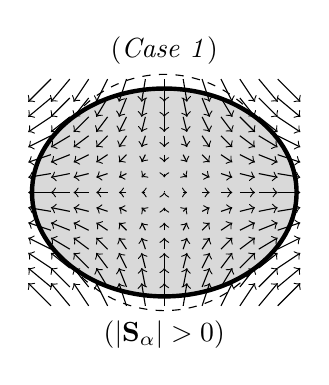
\begin{tikzpicture}[ultra thick,scale=0.6]
        \def\nRows{6}
        \def\nCols{6}
        \draw[dashed,thin] (0,0)circle(2.5);
        \draw[fill=gray!30] (0,0)ellipse(2.8 and 2.2);
        \foreach \x in {-\nRows,...,\nRows} {
            \foreach \y in {-\nCols,...,\nCols} {
                \pgfmathsetmacro\distance{veclen(\x*0.4, \y*0.4)};
                \pgfmathparse{\distance < 2.45 ? "blue" : "white"}
                \edef\colour{\pgfmathresult};
                \ifthenelse{\equal{\colour}{blue}}{                    
                    \draw[thin,->](\x*0.4,\y*0.4)--++(0.08*\x,-0.08*\y);
                }
            }
        }
        \node (txt) at (0,3){(\textit{Case 1})};
        \node (txt) at (0,-3){($|\textbf{S}_\alpha| > 0$)};
    \end{tikzpicture}
     \hfill
    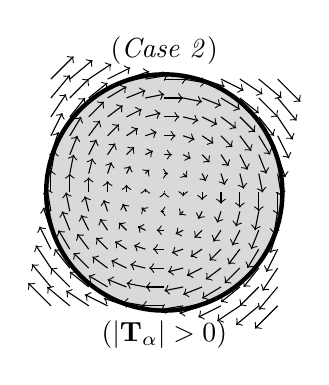
\begin{tikzpicture}[ultra thick,scale=0.6]
        \def\nRows{6}
        \def\nCols{6}
        \draw[fill=gray!30] (0,0)circle(2.5);
        \foreach \x in {-\nRows,...,\nRows} {
            \foreach \y in {-\nCols,...,\nCols} {
                \pgfmathsetmacro\distance{veclen(\x*0.4, \y*0.4)};
                \pgfmathparse{\distance < 2.5 ? "blue" : "white"}
                \edef\colour{\pgfmathresult};
                \ifthenelse{\equal{\colour}{blue}}{                    
                    \draw[thin,->](\x*0.4,\y*0.4)--++(0.08*\y,-0.08*\x);
                }
            }
        }
        \node (txt) at (0,3){(\textit{Case 2})};
        \node (txt) at (0,-3){($|\textbf{T}_\alpha| > 0$)};
    \end{tikzpicture}
    \hfill
    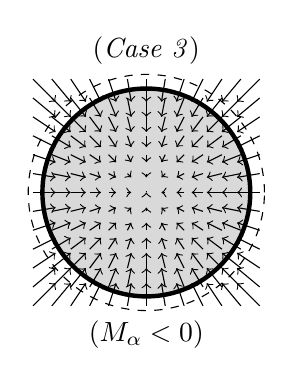
\begin{tikzpicture}[ultra thick,scale=0.6]
        \def\nRows{6}
        \def\nCols{6}
        \draw[dashed,thin] (0,0)circle(2.5);
        \draw[fill=gray!30] (0,0)circle(2.2);
        \foreach \x in {-\nRows,...,\nRows} {
            \foreach \y in {-\nCols,...,\nCols} {
                \pgfmathsetmacro\distance{veclen(\x*0.4, \y*0.4)};
                \pgfmathparse{\distance < 2.3 ? "blue" : "white"}
                \edef\colour{\pgfmathresult};
                \ifthenelse{\equal{\colour}{blue}}{                    
                    \draw[thin,->](\x*0.4,\y*0.4)--++(-0.08*\x,-0.08*\y);
                }
            }
        }
        \node (txt) at (0,3){(\textit{Case 3})};
        \node (txt) at (0,-3){($M_\alpha < 0$)};
    \end{tikzpicture}
    \hfill
    \caption{Graphical representation of the inner kinematics   of an arbitrary particle under three scenarios. 
        The arrows represent the velocity field inside the particle, $\textbf{w}_d^0$, with the corresponding value of the moment of momentum tensor indicated below. 
        The operator $|\ldots|$ refers to the norm of the tensors. 
        According to the inner velocity field:
        (\textit{Case 1}) The particle experiences a mean rate of deformation, resulting in non-zero stretching of momentum along the principal axis of deformation;
        (\textit{Case 2}) The particle is rotating, leading to a non-zero angular momentum vector in the direction of rotation;
        (\textit{Case 3}) The particle undergoes compression, resulting in a negative trace of the moment of momentum.
    }
    \label{eq:scheme}
\end{figure}


All these quantities obey conservation laws that are given according to \ref{eq:avg_hybrid_q}, \ref{eq:avg_hybrid_q_1} and \ref{eq:avg_hybrid_q_n}, and read, 
\begin{align}
    m_p(\pddt + \textbf{u}_p \cdot \grad)n_p
    &=
    - n_p \div \textbf{u}_p\\
    n_p (\pddt + \textbf{u}_p \cdot \grad) \textbf{M}_p
    +\div  \pavg{\textbf{u}_\alpha'\textbf{M}_\alpha}
    &=
    n_p2  \textbf{S}_p
    \label{eq:dt_hybrid_Mp}\\
    \label{eq:dt_hybrid_up}
    m_p n_p(\pddt + \textbf{u}_p \cdot \grad)\textbf{u}_p
    + \div \pavg{m_p \textbf{u}_\alpha'\textbf{u}_\alpha'}
    &=
    m_p n_p \textbf{g}
    + \pSavg{\bm\sigma_f^0 \cdot \textbf{n}}\\
    \label{eq:dt_hybrid_mup}
    n_p (\pddt + \textbf{u}_p \cdot \grad) \bm{\mu}_p
    +\div  \pavg{\textbf{u}_\alpha'\bm\mu_\alpha}
    &=
    \pSavg{\textbf{r}\times(\bm\sigma_f^0\cdot \textbf{n}_d)}
    \\
    \label{eq:dt_hybrid_Sp}
    n_p (\pddt + \textbf{u}_p \cdot \grad) \textbf{S}_p
    +\div  \pavg{\textbf{u}_\alpha'\textbf{S}_\alpha}
    &=
    \rho_d \pOavg{
        \textbf{w}_d^0  \textbf{w}_d^0 
        -\frac{1}{3} (\textbf{w}_d^0 \cdot  \textbf{w}_d^0) \bm\delta
    }
    -2 \mu_d \pOavg{\textbf{e}_d^0} \nonumber \\
    &+\pSavg{\frac{1}{2}(\textbf{r}\bm\sigma_f^0+\bm\sigma_f^0\textbf{r}-\frac{2}{3}(\bm\delta_f^0 \cdot \textbf{r})\bm\delta)\cdot \textbf{n}_d}\nonumber\\
    &-  \pSavg{\gamma (\frac{1}{3}\bm\delta - \textbf{nn})}
    % + (1-\lambda)&\pOavg{2\mu_f\textbf{E}_f}
    % + \frac{1}{2}\pOavg{\textbf{r}(\div\bm\Sigma_f)+ (\div\bm\Sigma_f) \textbf{r}}
\end{align}
In these equations we have introduced $\textbf{e}_k^0 = \grad \textbf{u}_k^0 + \grad \textbf{u}_k^0$ as the local shear rate of phase $k$.
It is now clear that if the surface tension forces play no role in the linear and angular momentum equation, however, it impacts the moment of momentum $\textbf{P}_\alpha$ or more specifically its symmetric part $\textbf{S}_\alpha$.
Thus, the surface tension force impacts the hydrodynamic behavior of a particle solely through its action on $\textbf{S}_\alpha$, which is related to the shape of a particle represented by $\textbf{M}_\alpha$, through \ref{eq:dt_M_alpha}.
In \ref{ap:Moments_equations} we show how to derive the higher-order moment of momentum equations, which can also be viewed as formulas for the higher moments of the internal particle stress distribution. 
It is interesting to mention that in a recent study of \citet{dolata2021faxen} and \citet{zhou2020lamb} they make use of the first two moments of momentum equations hidden into another but equivalent form, valid in the Stokes flow regime. 
% In these expressions we partitioned the local hydrodynamic stress $\bm\sigma_f^0$ and $\bm\sigma_d^0$, into their fluctuating parts, $\bm\sigma_f'=\bm\sigma_f^0 - \bm\Sigma_f$,  $\bm\sigma_d' = \bm\sigma_d^0 + p_f\bm\delta - 2\mu_d \textbf{E}_f$ and mean parts $\bm\Sigma_f$ and $-p_f \bm\delta + 2\mu_d \textbf{E}_f$, respectively. 
% Note that one can also write these equations in terms of $\bm\Sigma$ and $\textbf{E}$, the only requirement being that the exchange terms of \ref{eq:dt_hybrid_Mp} to \ref{eq:dt_hybrid_Sp} must correspond to the exchange terms used in the continuous phase momentum conservation \eqref{eq:dt_uf} (with \ref{eq:def_sigma_eff_f} or \ref{eq:def_sigma_eff_f2}). 



Now let us turn our attention to the averaged momentum equation of the continuous phase. 
By application of \ref{eq:dt_f_k} for $f_k = \rho_f$ and $\textbf{u}_f\rho_f$ we obtain straightforwardly, the mass and momentum equation of the continuous phase under the two fluid formulation, 
\begin{align}
    (\pddt + \textbf{u}_f\cdot \grad)\textbf{u}_f&=-\phi_f \div \textbf{u}_f\\
    \phi_f \rho_f(\pddt + \textbf{u}_f  \cdot \grad) \textbf{u}_f
    % +  \div \avg{\chi_f\rho_f \textbf{u}_f'\textbf{u}_f'}
    &= 
    \div [\phi_f \bm\sigma_f-  \avg{\chi_f\rho_f \textbf{u}_f'\textbf{u}_f'}]
    + \phi_f \rho_f \textbf{g}
    - \avg{\delta_\Gamma \bm\sigma_f'\cdot \textbf{n}},
    \label{eq:two_fluid_momentum_init}
\end{align}
respectively. 
To obtain the hybrid formulation one may use \ref{eq:f_exp} to taylor expand the last term on the right-hand side of \ref{eq:two_fluid_momentum_init}. 
However, it is first important to discuss the form of the term $\phi_f\bm\sigma_f$ since a dispersed phase term, is hidden into it, hence it is important to identify this term before carrying out the Taylor expansion. 

\subsection{Mean stress formulation and momentum transfer decomposition}


The starting point is to note that $\phi_f\bm\sigma_f$ can be expressed in terms of the averaged fluid pressure $p_f$, and continuous phase averaged velocity ($\textbf{u}_f$), or bulk-averaged velocity ($\textbf{u} = \phi_f \textbf{u}_f + \phi_d \textbf{u}_d$).
Choosing to express $\bm\sigma_f$ as a function $\textbf{u}_f$ rather than $\textbf{u}$ and vice versa, results in two distinct forms of the momentum equation and two distinct formulations of the closure terms. 
Because it seems a bit unclear in the literature, we propose here to expose both formulations and discuss which of the two equivalent (but different) formulation is the most suited for multiphase flow modeling. 


First let us introduce what we call here the \textit{mean Newtonian stress}, based either on the bulk velocity \textbf{u} or on the continuous phase averaged velocity $\textbf{u}_f$, namely,
\begin{align}
    \bm\Sigma_f 
    &
    = -p_f \bm\delta + 2\mu_f \textbf{E}_f    
    = -p_f \bm\delta + \mu_f [\grad \textbf{u}_f + (\grad \textbf{u}_f)^{\dagger}], 
    \\
    \bm\Sigma &
    = -p_f\bm\delta + 2 \mu_f \textbf{E}
    = -p_f \bm\delta + \mu_f [\grad \textbf{u} + (\grad \textbf{u})^{\dagger}],
\end{align}
where \textbf{E} and $\textbf{E}_f$ represent the \textit{mean shear rate} based either on $\textbf{u}_f$ or on \textbf{u}. 
Using the constitutive law of Newtonian fluids we find, 
\begin{align}
    \phi_f \bm\sigma_f 
    &=
    % - \phi_f p_f \bm\delta
    % + \phi_f \mu_f [\grad \textbf{u}_f  + (\grad \textbf{u}_f)^\dagger]
    % - \mu_f \avg{\delta_\Gamma( \textbf{u}_f'  \textbf{n}_d +  \textbf{n}_d \textbf{u}_f' )}
    % =
    \phi_f \bm\Sigma_f
    - \mu_f \avg{\delta_\Gamma( \textbf{u}_f'  \textbf{n}_d +  \textbf{n}_d \textbf{u}_f' )}
    \label{eq:stress_closure}\\
    \phi_f \bm\sigma_f 
    &=
    % - \phi_f p_f \bm\delta
    % + \mu_f [\grad \textbf{u}  + (\grad \textbf{u})^\dagger]
    % - 2\mu_f \phi_d \textbf{e}_d
    % =
    \phi_f \bm\Sigma
    - \avg{2\mu_f \chi_d \textbf{e}_d'}
    \label{eq:stress_closure1}
\end{align}
where we have used the relations 
\begin{equation}
    \avg{\chi_f \grad \textbf{u}_f^0}
    = 
    \phi_f \div  \textbf{u}_f
    + \avg{\delta_\Gamma \textbf{n}_f \textbf{u}_f'}
    \label{eq:first_rel}
\end{equation}
and
\begin{equation}
    \avg{\chi_f \textbf{e}_f^0}
    = 
    \avg{\textbf{e}^0}
    - \avg{\chi_d \textbf{e}_d^0}
    = 
    \textbf{E}
    - \avg{\chi_d \textbf{e}_d^0}
    = 
    \phi_f \textbf{E}
    - \avg{\chi_d \textbf{e}_d^*},
    \label{eq:sec_rel}
\end{equation}
to derive \ref{eq:stress_closure,eq:stress_closure1}, respectively. 
Note that \ref{eq:first_rel} is true unconditionally, while \ref{eq:sec_rel} requires the condition that there is no shear stress at the interface of the droplets, so that $\avg{\delta_\Gamma \textbf{e}_\Gamma^0}= 0$, which is true in most of the practical cases of interest. 
In \ref{eq:stress_closure1} we have introduced $\textbf{e}_d^* = \textbf{e}_d^0 - \textbf{E} = \grad (\textbf{u}_d^0-\textbf{u})+\grad (\textbf{u}_d^0-\textbf{u})^\dagger$ which is the droplet internal shear rate relative to the `bulk' shear rate \textbf{E}.
While $\textbf{u}_f' = \textbf{u}_f^0 - \textbf{u}_f$ in \ref{eq:stress_closure}. 


Before presenting the hybrid form of the continuous phase momentum equation, it is interesting to expose the classic two-fluid formulation using the stress formulation given by \ref{eq:stress_closure1} in the first place. 
The momentum averaged equations read, 
\begin{align}
    % (\pddt + \textbf{u}_f\cdot \grad)\textbf{u}_f&=-\phi_f \div \textbf{u}_f\\
    \phi_f \rho_f(\pddt + \textbf{u}_f  \cdot \grad) \textbf{u}_f
    % +  \div \avg{\chi_f\rho_f \textbf{u}_f'\textbf{u}_f'}
    &= \phi_f 
    \left(\div \bm{\Sigma}_f
    + \rho_f \textbf{g}\right)
    - \div 
    [\avg{\chi_f\rho_f \textbf{u}_f'\textbf{u}_f'}
    +\avg{\delta_\Gamma \mu_f( \textbf{u}_f'  \textbf{n}_d +  \textbf{n}_d \textbf{u}_f')}]
    - \avg{\delta_\Gamma \bm\sigma_f^*\cdot \textbf{n}},
    \label{eq:two_fluid_momentum}
\end{align}
where, $\bm\sigma_f^*=\bm\sigma_f^0 - \bm\Sigma_f$ is the Newtonian stress evaluated at a point on an interface relative to the mean stress $\bm\Sigma_f$. 
Likewise, using \ref{eq:stress_closure1} one may also derive another form of the momentum equation, namely,
\begin{equation}
    \phi_f \rho_f(\pddt + \textbf{u}_f  \cdot \grad) \textbf{u}_f
    % +  \div \avg{\chi_f\rho_f \textbf{u}_f'\textbf{u}_f'}
    = \phi_f 
    \left(\div \bm{\Sigma}
    + \rho_f \textbf{g}\right)
    - \div 
    [\avg{\chi_f\rho_f \textbf{u}_f'\textbf{u}_f'} + \avg{2\mu_f \chi_d \textbf{e}_d'}]
    - \avg{\delta_\Gamma \bm\sigma_f^*\cdot \textbf{n}},
    \label{eq:two_fluid_momentum2}
\end{equation} 
In this new formula it is implied that $\bm\sigma_f^*=\bm\sigma_f^0 - \bm\Sigma$.
Clearly, subtracting by $\bm\Sigma_f$ to the local stress at the interface leads to the expression 
\begin{equation}
    \bm\sigma_f^* 
    =
    -p_f'\bm\delta
    + \mu_f [
        \grad \textbf{u}_f'
        + ^\dagger \grad \textbf{u}_f'
    ]
    \label{eq:disturbance_stress}
\end{equation}
which corresponds to the Newtonian stress at the surface of the droplets (relative to the mean pressure and velocity field) typically available in numerical or theoretical studies.
Likewise, substituting the mean stress with $\bm\Sigma$ in \ref{eq:disturbance_stress} one obtain the same formula except than $\textbf{u}_f'\to \textbf{u}_f^0 - \textbf{u}$. 
Hence, in both case one has to compute the local stress relative to the averaged continuous phase motion or bulk phase motion. 
% Note that because $\div \textbf{u} = 0$ it may be more convenient to  




The last two terms on the right-hand side of \ref{eq:two_fluid_momentum} can be further expanded into a Taylor series using \ref{eq:f_exp_delta}. 
Doing so leads us to the hybrid formulation of the continuous phase momentum  equation (i.e. \ref{eq:avg_hybrid_dt_chi_f} with $f_f^0 = \textbf{u}_f^0\rho_f$), namely,
\begin{align}
    \phi_f \rho_f(\pddt + \textbf{u}_f  \cdot \grad) \textbf{u}_f
    &= \phi_f 
    \left(\div \bm{\Sigma}_f
    + \rho_f \textbf{g}\right)
    + \div \bm\sigma_f^\text{eff}
    - \pSavg{\bm\sigma_f'\cdot \textbf{n}}, 
    \label{eq:dt_uf}
\end{align}
where we introduced the effective stress, 
\begin{align}
    \bm{\sigma}^{\text{eff}}_f 
    &= 
    - \avg{\chi_f\rho_f \textbf{u}_f'\textbf{u}_f'} 
    + \pSavg{[\textbf{r}\bm\sigma'_f\cdot \textbf{n} - \mu_f (\textbf{u}_f' \textbf{n} + \textbf{n} \textbf{u}_f')]}\nonumber\\
    &- \div
        \pSavg{[\frac{1}{2}\textbf{rr}\bm\sigma'_f\cdot \textbf{n}- \mu_f\textbf{r} (\textbf{u}_f' \textbf{n} + \textbf{n} \textbf{u}_f')]}
        + \grad\grad (\ldots)
    \label{eq:def_sigma_eff_f}
\end{align}
Alternatively, one may use \ref{eq:two_fluid_momentum2} as a starting point.
In this case we obtain a relation similar to \ref{eq:dt_uf} except that $\bm\Sigma_f$ is replaced by $\bm\Sigma$, and the effective stress $\bm\sigma_f^\text{eff}$ by the tensor
\begin{align}
    \bm{\sigma}^{\text{eff}} 
    &= 
    - \avg{\chi_f\rho_f \textbf{u}_f'\textbf{u}_f'} 
    + \pavg{\intO{\textbf{r}\bm\sigma'_f\cdot \textbf{n}} - \delta_p\intO{2\mu_f\textbf{e}_d'}}\nonumber\\
    &- \div
        \pavg{ \frac{1}{2}\intS{\textbf{rr}\bm\sigma'_f\cdot \textbf{n}}
        - \delta_p\intO{2\mu_f \textbf{r} \textbf{e}_d'}}
        + \grad\grad (\ldots). 
    \label{eq:def_sigma_eff_f2}
\end{align}
In this formulation it is implied that $\bm\sigma_f'$ is given by $\bm\sigma_f' = \bm\sigma_f^0 -\bm\Sigma$. 
Note that the differences between the formulation between \ref{eq:def_sigma_eff_f2} and \ref{eq:def_sigma_eff_f} plus the differences between the corresponding drag force terms, is exactly equal to, $\phi_f (\div \bm\Sigma_f - \div\bm\Sigma)$.
Hence, the transition from one formulation to the other is straightforward, it just requires adding or subtracting $\phi_f (\div \bm\Sigma_f - \div\bm\Sigma)$. 


Under this form, the left-hand side of \ref{eq:dt_uf} represents the total derivative of $\textbf{u}_f$, while on the right-hand side we find: (1) the mean Newtonian contribution $\bm\Sigma_f$ (or $\bm\Sigma$), (2) the mean buoyant force, (3) the Reynolds stress term, and (4) the moments of momentum exchange terms, which are computed based on $\bm\Sigma_f$ (or $\bm\Sigma$). 
% One can remark the similarities between the surface exchange terms expansion, and the multipole expansion used in microhydrodynamic that characterize the disturbance field caused by a body immersed in a stokes flow \citet{pozrikidis1992boundary,kim2013microhydrodynamics}. 
The last term of \ref{eq:dt_uf} corresponds to the mean hydrodynamic drag force on the particles.
Then one can wonder which of the formulation, \ref{eq:def_sigma_eff_f2} or \ref{eq:def_sigma_eff_f}, contains what is called the `Stresslet' and the higher moments of force given by the multipole expansion used in microhydrodynamic ? \citep{pozrikidis1992boundary,kim2013microhydrodynamics}\footnote{Note that the first term in this expansion is the same whether we use \ref{eq:def_sigma_eff_f2} or \ref{eq:def_sigma_eff_f}}.   
These moments are usually defined as the `extra stress above the value of the fluid law'\citep{hinch1977averaged}.
Because we are not studying the `bulk' momentum equation this definition does not directly apply in our context. 
However, note that \ref{eq:stress_closure1} involves the bulk velocity \textbf{u} which must be used in the bulk stress momentum equation.
Hence, we can state that the resulting formulation based on \ref{eq:stress_closure1} and given by \ref{eq:def_sigma_eff_f2}, corresponds to the multipole expansion of microhydrodynamic. 
\tb{not entirely sure but i think this is an important point }
Thus, the symmetric part of the second term of \ref{eq:def_sigma_eff_f2} is exactly what is called the `Stresslet', while the skew-symmetric part represents the hydrodynamic torque applied on the droplets.
The remaining terms of \ref{eq:def_sigma_eff_f2} represent the contribution of the second, third\ldots, and higher moments of hydrodynamic forces acted upon the droplets.  

As a side note, remark that the second order and higher moments in \ref{eq:def_sigma_eff_f} (or \ref{eq:def_sigma_eff_f2}) appear under two divergence operators in \ref{eq:dt_uf}. 
Hence, if we note $\Sigma_{ijk}$ the third rank tensor that represent these moments, then only the vector $\partial_k \partial_j\Sigma_{ijk}$ is of physical significance in the momentum balance \eqref{eq:def_sigma_eff_f}.
Thus, one can demonstrate that \citep{lhuillier1996contribution}
\begin{equation}
    \partial_j \partial_k \Sigma_{ijk}
    = \partial_j \partial_k \Sigma_{i(jk)}
    =
    \partial_j \partial_k \left[
        \Sigma_{i(jk)}
        + \Sigma_{j(ik)}
        - \Sigma_{k(ij)}
    \right],
    \label{eq:sym_proof}
\end{equation}
where $\Sigma_{i(jk)} = \frac{1}{2}[\Sigma_{ijk} + \Sigma_{ikj}]$ represents the symmetric part of $\Sigma_{ijk}$ over the index $jk$, as indicated by the parenthesis (and so on for the other tensor). 
This expression is allowed because $\partial_j \partial_k (\Sigma_{ijk} - \Sigma_{ikj}) = 0$ and $\partial_j \partial_k (\Sigma_{j(ik)} - \Sigma_{k(ij)}) = 0$. 
This manipulation highlight the fact that the effective stress due to the second order moments remains symmetric over the indices $ij$, in all circumstances.
Hence, as already demonstrated by \citet{lhuillier1996contribution} only the hydrodynamic torque can induce skew-symmetric stresses in \ref{eq:dt_uf}. 




This set of equations are completed by a condition on the total volume conservation which reads, 
\begin{equation}
    \phi_f + \phi_d = 
    \phi_f +  n_pv_p + \frac{1}{2}\grad\grad : (\textbf{M}_p n_p) + \ldots = 1. 
    \label{eq:volume_conservation}
\end{equation}
Because $\textbf{u}$ may be required by \ref{eq:stress_closure1}, one also need to solve the equation, 
\begin{equation}
    \textbf{u} = \textbf{u}_f\phi_f + 
    n_pv_p\textbf{u}_p + \div  (\textbf{P}_p n_p) + \ldots
    \label{eq:velocity_conservation}
\end{equation}

Even though, both stress decomposition and momentum formulations proposed here are equivalent, each formulation have advantages and drawback which we discuss below.  
Additionally, because other stress decomposition are already proposed in the literature we propose to discuss first of their advantages and draw back. 


In the pioneering study of \citep{zhang1997momentum}, and in numerous articles that followed, the disturbance stress is defined as $\bm\sigma_f'= \bm\sigma_f^0 - \bm\sigma_f$ which is what we could call the ``intuitive'' definition. 
However, note that using \ref{eq:stress_closure} one obtain that, 
\begin{equation}
    \bm\sigma_f'
    =
    -p_f'\bm\delta
    + \mu_f [
        \grad \textbf{u}_f'
        + ^\dagger \grad \textbf{u}_f'
    ]
    + \frac{\mu_f}{\phi_f} \avg{\delta_\Gamma( \textbf{u}_f'  \textbf{n}_d +  \textbf{n}_d \textbf{u}_f' )}
    \label{eq:stress_closure_zhang}
\end{equation}
The first two terms of this expression correspond to the relative Newtonian stress usually integrated on the surface of a droplet or solid particle.
The last term is one of the contributions related to the dispersed phase which normally appear in the effective stress expansion as shown above. 
Same comments apply if one consider \ref{eq:stress_closure1} in the above expression. 
Hence, because $\bm\sigma_f$ already contains closure terms related to the dispersed phase, it felt unnecessarily complicated to subtract the whole expression of $\bm\sigma_f$ from $\bm\sigma_f^0$.
Nevertheless, note that because the last term of \ref{eq:stress_closure_zhang} is at most of $\mathcal{O}(\phi)$, the total contribution from this term when integrated on the droplets surface becomes of $\mathcal{O}(\phi^2)$, hence it can be safely neglected in dilute regime. 

One may also consider using $p_f\bm\delta$ instead of $\bm\sigma_f$, $\bm\Sigma_f$ or $\bm\Sigma$, as done in \citet{morel2015mathematical} (\tb{paper de daniel ou il fait ca ?}), in this case $\bm\sigma_f'  = -p_f' \bm\delta + \mu_f (\grad \textbf{u}_f^0 + ^\dagger \grad \textbf{u}_f^0)$, hence the closure are computed based on the absolute local velocity $\textbf{u}_f^0$ instead of $\textbf{u}_f'$.
Without going into the details, note that numerous drag force closures are based on the reciprocal theorem formulation, this includes the expressions given by the famous Faxen laws.
The closures (drag forces, stresslet etc... ) provided by the reciprocal theorem are by construction expressed in terms of the disturbance fields ($p_f'$,$\textbf{u}_f'$), because they must decay to zero far from the test particle. 
Therefore, this last formulation may not be the most practical as well\footnote{
For example, the Faxen contribution to the drag force, given by $\textbf{f} = \pi a^3 \mu_f \grad^2 \textbf{u}_f$ only considers the contribution from the disturbance stress, $\bm\sigma_f'  = -p_f' \bm\delta + \mu_f (\grad \textbf{u}_f' + ^\dagger \grad \textbf{u}_f')$, which vanish far from the test particle. 
If one uses the formulation based on $\bm\sigma_f'  = -p_f' \bm\delta + \mu_f (\grad \textbf{u}_f^0 + ^\dagger \grad \textbf{u}_f^0)$, the Faxen contribution to the drag force becomes $\textbf{f} = \pi a^3 \mu_f \grad^2 \textbf{u}_f + \frac{4\pi a^3}{3}\mu_f \grad^2 \textbf{u}_f$ where the second term is the contribution from the mean velocity field.
Although both formulations are equally valid, the second one appears to be less commonly used and could potentially lead to misinterpretations or inconsistencies if not carefully handled. 
}. 


Now let us discuss on the choic between $\bm\Sigma$ and $\bm\Sigma_f$. 
At first sight, using \ref{eq:dt_uf} with the effective stress given by \ref{eq:def_sigma_eff_f}, seems more practical because we are solving for the field $\textbf{u}_f$ hence avoiding the need of \ref{eq:velocity_conservation}. 
On the other hand we note that for solid particles $\textbf{e}_d^0 = 0$ and $\avg{\chi_d \textbf{e}_d'} = -\bm\Sigma\phi_d$, because of this great simplification \ref{eq:stress_closure1} is often used \citep{jackson2000} even if it requires adding \ref{eq:velocity_conservation} in the system of equation.  
But there is another reason for using the `bulk stress' $\bm\Sigma$ as a reference stress to compute the closure terms involving $\bm\sigma_f'$. 
Indeed, since $\bm\sigma_f'$ requires $\textbf{u}_f' = \textbf{u}_f^0 - \textbf{u}$, then \textbf{u} becomes the `far field' or `undisturbed' velocity boundary condition far from the test particle in the conditionally averaged Navier-Stokes equations \tb{(+my phd)}.
On another hand, one may note that all the available theoretical solutions considering the disturbance field of a particle embedded in a pure solvent or in an effective medium (which represents other particles' contribution) use a divergence free `background flow' as limiting condition \citep{kim1985modelling,hinch1977averaged}.
Since $\div \textbf{u} =0$ we deduce that the velocity field used in most (if not all) theoretical problems correspond to \textbf{u}. 
Therefore, the disturbance  stress computed in these problems is $\bm\sigma_f'= \bm\sigma_f^0 - \bm\Sigma$. 
In opposition, the stress decomposition based on $\bm\Sigma_f$, involves the fields $\textbf{u}_f$ which is not divergence free. 
Hence, this `far field' or `undisturbed' velocity boundary condition far from the test particle does not correspond to the usual boundary condition assumed in most of the theoretical problems. 
In conclusion, it is important to note that \textbf{u} corresponds exactly to the `background velocity' fields used in most of the theoretical derivations.
Hence, the resulting closure terms (drag forces, stresslet and higher moments) derived in these studies refer to the closures expressed in terms of $\bm\sigma_f^0 - \bm\Sigma$.
In all case one can always express $\bm\Sigma_f$ in terms of $\bm\Sigma$ hence which formulation to use is not a fatality. 
However, one must always be careful when asserting that a given formulation of the drag force, for example, is exactly equivalent to a closure term found in the literature, as there are multiple possible formulations  (either based on $\bm\Sigma_f$, $\bm\Sigma$, $\bm\sigma_f$ or even  $p_f \bm\delta$). 
Note that the choices between $\bm\Sigma_f$ and $\bm\Sigma$ only matter if one consider a closure problem, in which $\phi \textbf{u}_f \neq \phi \textbf{u}$, hence accurate at $\mathcal{O}(\phi^2)$ at least (such as in \citet{hinch1977averaged,kim1985modelling}). 


Because of this last remark, we will use in the following the formulation based on $\bm\Sigma_f$ (i.e. \ref{eq:dt_uf} and \ref{eq:def_sigma_eff_f}) since we are working at $\mathcal{O}(\phi)$.
This will avoid the need for \ref{eq:velocity_conservation} in the system of equation. 
\tb{on pourrait utiliser aussi lautre peut importe }



\subsection{Closure in viscous dominated flows for dilute suspension}

The closure terms in the above set of equation are expressed in terms of $p_f'$ and $\textbf{u}_f'$, therefore we are seeking for the disturbance velocity and pressure fields generated by a spherical droplet immersed in an arbitrary flow. 
Specifically, the fields $(\textbf{u}_f',p_f')$ correspond to the solution of the 
 \textit{single-particle conditionally averaged} Navier-Stokes equations \citep{hinch1977averaged,zhang1994averaged} \tb{(+ my phd)}. 
Note that to obtain a solution accurate at $\mathcal{O}(\phi)$ to these equations, it is sufficient to consider a closure problem accurate at $\mathcal{O}(\phi^0)$\citep{hinch1977averaged,zhang1994averaged}.
Additionally, we neglect inertia in the closure problem, meaning that we neglect all the terms of $\mathcal{O}(Re)$ in the closure problem, and all the term of $\mathcal{O}(Re\phi)$ in the averaged equations. 
Consequently, we consider an isolated spherical droplet translating in an arbitrary Stokes flow.
The solution for this problem can be found in many studies in the literature, including \citet{leal2007advanced,pozrikidis1992boundary,kim2013microhydrodynamics,pozrikidis2011introduction,nadim1991motion} which will enable us to compute the closure terms.

\subsubsection{Hydrodynamic stresses closures at $\mathcal{O}(\phi Re^0 Ca^0)$}
In the first place we focus on the surface exchange terms. 
We may directly compute the following expressions from the singularity solutions and find, 
\begin{align}
    \pSavg{\bm\sigma_f^*\cdot \textbf{n}} &
    =
    \phi
    \frac{\mu_f}{a^2}
    \frac{3(2+3\lambda)}{2(1+\lambda)}\textbf{u}_r
    + \phi\mu_f  \frac{3\lambda}{4(\lambda +1)} \grad^2 \textbf{u}_f
    % + \phi \frac{1}{a}\frac{1}{\lambda +1} \grad \gamma
    % + \phi a \frac{1}{10(\lambda +1)}\grad^2(\grad\gamma)
    \label{eq:drag_forces}
    \\
    \pSavg{\textbf{r}\bm\sigma_f^*\cdot \textbf{n}} &
    = \mu_f \phi 
    \frac{3(5\lambda +2)}{5(\lambda +1)}\textbf{E}_f
    + \mu_f a^2 \phi \frac{3\lambda}{10(\lambda+1)}\grad^2  \textbf{E}_f
    % + \phi a \frac{9}{25(\lambda +1)}\grad\grad \gamma
    % - \phi a \frac{3}{25(\lambda +1)}\bm\delta\grad^2 \gamma
    \\
    \pSavg{\textbf{rr}\bm\sigma_f^*\cdot \textbf{n}} &
    =
    \mu_f \phi \frac{3}{5(\lambda +1)} (\textbf{u}_r \bm\delta + \bm\delta \textbf{u}_r)
    + \mu_f \phi \frac{3(5\lambda +2)}{10(\lambda+1)}\bm\delta \textbf{u}_r
    \\
    % &+ a^2 \mu_f \phi \frac{119\lambda^2+190\lambda-24}{140(\lambda+1)(\lambda+4)}(\grad\grad \textbf{u}_f)_{jki}
    % + a^2\mu_f \phi \frac{7\lambda^2+190\lambda+88}{140(\lambda+1)(\lambda+4)}\grad(\grad \textbf{u}_f+\grad \textbf{u}_f^\dagger )_{ijk}\nonumber\\
    % &+a^2\mu_f \phi \frac{13\lambda - 4 }{14(\lambda+1)(\lambda+4)}\grad^2 ( \textbf{u}_f\bm\delta)_{ijk}
    % - a^2\mu_f \phi \frac{7\lambda^2 + 80 \lambda - 72}{140(\lambda+1)(\lambda+4)}\grad^2(\textbf{u}_f\bm\delta  + \textbf{u}_f \bm\delta)_{jki}\nonumber \\
    % \pSavg{\textbf{rrr}\bm\sigma_f'\cdot \textbf{n}} &
    % =
    % a^2\phi\frac{4}{105}\frac{21\lambda+2}{\lambda+1}
    % (\textbf{E}\bm\delta+\textbf{E}\bm\delta + \textbf{E}\bm\delta)
    % + 
    % a^2\phi \frac{64}{105(\lambda+1)}
    % (\bm\delta\textbf{E}+\bm\delta\textbf{E} + \bm\delta\textbf{E})
\end{align}
\begin{align}
    \pSavg{ (\textbf{n} \textbf{u}_f' + \textbf{u}_f' \textbf{n})}
    &=
    -  \phi \frac{2(5\lambda +2)}{5(\lambda+1)}\textbf{E}_f
    -  a^2 \phi \frac{3\lambda}{15(\lambda+1)}\grad^2  \textbf{E}_f
    % - \phi a  \frac{6}{25(\lambda+1)} \grad\grad \gamma
    % + \phi a \frac{2}{25(\lambda+1)} \bm\delta\grad^2 \gamma\\
    \\
    \pSavg{ \textbf{r}(\textbf{n} \textbf{u}_f' + \textbf{u}_f' \textbf{n})}
    &=
    -\phi \frac{10\lambda +7}{10(\lambda+1)}
    (\bm\delta \textbf{u}_r + \textbf{u}_r \bm\delta)
    - \phi  \frac{1}{5(\lambda+1)}\bm\delta \textbf{u}_r
    % &-  a^2 \phi \frac{2(2\lambda+1)}{7(\lambda+1)(\lambda+4)}(\grad\grad \textbf{u}_f)_{ijk}
    % - a^2 \phi \frac{7\lambda^2+20\lambda+3}{35(\lambda+1)(\lambda+4)}\grad(\grad \textbf{u}_f+\grad \textbf{u}_f)_{kij}\nonumber\\
    % &+ a^2 \phi \frac{3\lambda-2}{14(\lambda+1)(\lambda+4)}\grad^2(\bm\delta\textbf{u}_f)_{ijk}
    % -  a^2 \phi \frac{14\lambda^2+75\lambda+6}{140(\lambda+1)(\lambda+4)}\grad^2 (\textbf{u}_f \bm\delta + \textbf{u}_f \bm\delta)_{ijk}\nonumber
    \label{eq:secondUN}
    % \pSavg{ \textbf{rr}_{mq}(\textbf{n} \textbf{u}_f' + \textbf{u}_f' \textbf{n})_{iv}}
    % &=
    % -\phi a^2 \frac{4(7\lambda+4)}{105(\lambda+1)}
    % (\textbf{E}_{im} \bm\delta_{qv}
    % +\textbf{E}_{iq}\bm\delta_{mv}
    % + \textbf{E}_{mv} \bm\delta_{iq}
    % + \textbf{E}_{qv}\bm\delta_{im}
    % )
    % \\
    % &
    % -\phi a^2 
    % \frac{16}{105(\lambda+1)}(\textbf{E}_{mq}\bm\delta_{iv})
    % -\phi a^2 \frac{8(7\lambda+2)}{105(\lambda+1)}\textbf{E}_{iv}\bm\delta_{mq}
    % \label{eq:thirsmom}
\end{align}
where we have introduced the relative velocity $\textbf{u}_r = \textbf{u}_f - \textbf{u}_p$, and the viscosity ratio $\lambda = \mu_d/\mu_f$. 
Note that we have used the approximation $\phi=n_pv_p + \mathcal{O}(a^2/L^2)$ and remove any terms of $\mathcal{O}(a^3/L^3)$ or higher (where $L$ corresponds to the typical length  scale of variation of the mean quantities). 

\tb{
    Because 
    \begin{align}
        \pSavg{ \textbf{r}(\textbf{n} \textbf{u}_f' + \textbf{u}_f' \textbf{n})}
        &=
        \pOavg{ \grad(\textbf{r}\textbf{u}_f') + \div(\textbf{u}_f' \textbf{r})}\\
        &=
        \pOavg{ \textbf{r} \textbf{e}_d'}
        +\pOavg{ \bm\delta \textbf{u}_f' + \textbf{u}_f' \bm\delta}\\
        &=
        \pOavg{ \textbf{r} \textbf{e}_d'}
        +\phi (\textbf{u}_r \bm\delta 
        + \bm\delta \textbf{u}_r)  \\
    \end{align}
    one can easily recover the other closure formulaiton
}

The above closure just provide the contribution from the disturbance fields, however in the dispersed phase relations \eqref{eq:dt_hybrid_up,eq:dt_hybrid_Sp} one need the contribution from the total stress $\bm\sigma_f^* +\bm\Sigma_f$ that will be needed in the dispersed phase equations , can be expressed as\citep{zhang1997momentum,morel2015mathematical}, 
\begin{align}
    \pSavg{\bm\sigma_f^0}
    =
    \pSavg{\bm\sigma_f^*}
    + \pOavg{\div\bm\Sigma_f} 
    &= 
    \pSavg{\bm\sigma_f^*}
    + \phi\div\bm\Sigma_f  
    % +\frac{1}{2\rho_d}\textbf{M}_p:\grad\grad\div\bm\Sigma_f 
    % \\
    % \pOavg{2\textbf{E}_f} 
    % &= 2\phi\textbf{E}_f 
    % +
    % \frac{1}{\rho_d }\textbf{M}_p :\grad\grad \textbf{E}_f
    % \\
    % \pOavg{\textbf{r}\div\bm\Sigma_f} 
    % &= 0
    % \frac{1}{\rho_d}(\textbf{M}_p\cdot
    % \grad) (\div\bm\Sigma_f )
    \label{eq:mean_contributions}
\end{align}
where we have used the approximation of $\bm\Sigma_f(\textbf{x}+\textbf{r}) = \bm\Sigma_f(\textbf{x}) + \textbf{r}\cdot\grad \bm\Sigma_f|_{\textbf{r}=0}$ and neglected the $\mathcal{O}(a^2/L^2)$ terms. 
Others similar expressions can be used for the integral of $\textbf{r}\bm\sigma_f^0\cdot \textbf{n}$, and the volume integral of $\textbf{e}_d^0$ in \ref{eq:dt_hybrid_Sp}. 


\subsubsection{Velocity variance and covariance closures}


The disturbance velocity field $\textbf{u}_f'$ is proportional to $\propto \textbf{u}_r$, $\grad\textbf{E}_f$ and $\grad\grad \textbf{u}_f$.
Additionally, the Reynolds stress tensor $\avg{\chi_f \textbf{u}_f'\textbf{u}_f'}$ is a symmetric second-order tensor. 
We deduce that the functional form of the Reynolds stress must be 
\begin{multline}
    \avg{\chi_f \rho_f \textbf{u}_f' \textbf{u}_f'}
    =
    C_{uu}^1(\phi,\lambda) \rho_f \textbf{u}_{r} \textbf{u}_{r}
    + C_{uu}^2(\phi,\lambda) \rho_f (\textbf{u}_{r}\cdot  \textbf{u}_{r})\bm\delta\\
    +a^2 C_{EE}^1(\phi,\lambda) \rho_f\textbf{E}_f\cdot \textbf{E}_f 
    +  a^2 C_{EE}^2(\phi,\lambda) \rho_f (\textbf{E}_f : \textbf{E}_f)\bm\delta.
    + \ldots
    \label{eq:Reynolds_stress_functional_form}
\end{multline}
where the remaining terms indicated by the $\ldots$ represent linear combination of terms proportional to $a^4\grad\grad \textbf{u}_f:\grad\grad \textbf{u}_f$. 
The exact values for the $C_{EE}$ can be found in \citet{raja2010inertial}\tb{(+myphd)}, however as these terms are factors of $a^2$ they are of $\mathcal{O}(a^2/L^2)$, hence only the first two terms of \ref{eq:Reynolds_stress_functional_form} are relevant in the momentum equation. 
Because, the Reynolds stress term is an averaged quantity performed over the continuous phase domain ($\chi_f$), the disturbance fields $\textbf{u}_f'$ cannot be integrated to obtain the constant $C_{uu}^1$ and $C_{uu}^2$. 
However, note that according to these experimental\citep{cartellier2009induced}, numerical\tb{(+my phd)}, and theoretical\citep{hill2001first}\tb{(+my phd)} studies we may expect the relations $C_{uu}^1,C_{uu}^2 \propto \phi^{2/3} \frac{(2+3\lambda)^2}{(\lambda+1)^2}$. 


In the present context we neglected the droplets' interactions in the closure problem, hence we expect $\pavg{\textbf{u}_\alpha'\textbf{u}_\alpha'}=0$.
However, using symmetry arguments, and experimental result from the literature \citep{guazzelli2011fluctuations}, we arrive at the conclusion that, 
\begin{equation}
    \pavg{m_p \textbf{u}_\alpha'\textbf{u}_\alpha'}
    =
    \rho_d C^1_{up}(\phi,\lambda)\textbf{u}_r\textbf{u}_r
    + \rho_d C^2_{up}(\phi,\lambda) \bm\delta(\textbf{u}_r\cdot \textbf{u}_r)
    \label{eq:upup}
\end{equation}
where $C_{up}^1$ and $C_{up}^2$ are unknown constants which are $\propto \phi^{2/3}$\citep{guazzelli2011fluctuations}. 
This result shows that due to the long range interactions between the droplets, the particles' velocity variance, is non-zero even at $\mathcal{O(\phi)}$. 
Finally, note that both $\pavg{m_p \textbf{u}_\alpha'\textbf{u}_\alpha'}$ and $\avg{\rho_f \textbf{u}_f'\textbf{u}_f'}$, are by construction inertial contributions.
However, in dimensionless form both terms are $\propto \mathcal{O}(Re \phi^{2/3})$. 
Because,  $\mathcal{O}(\phi^{2/3}Re) > \mathcal{O}(Re\phi)$ we conclude that the velocity variance terms must be conserved even under the Stokes flow hypothesis in the averaged equations. 


The covariance terms on the left-hand side of \ref{eq:dt_hybrid_Mp} to \ref{eq:dt_hybrid_Sp}, witness of the correlation between the shape of the droplet ($\textbf{M}_\alpha$), its angular momentum ($\bm\mu_\alpha$), and its momentum of deformation ($\textbf{S}_\alpha$), with its center of mass velocity $\textbf{u}_\alpha$. 
If one of these properties is independent to the center of mass velocity, then the corresponding covariance term will vanish. 
In dilute Stokes regime, a translating spherical droplets remains spherical as the normal stresses on its surface are at equilibrium\citep{taylor1964deformation}. 
Likewise, a translating droplet does not undergo hydrodynamic torque, hence no angular momentum are produced by translation\footnote{At finite inertial effect these two statements are false, because of the well known Magnus effect, and because a spherical droplet undergo deformation due to its relative motion with the ambient fluid.}.
We deduce that in this restricted regime $\textbf{M}_\alpha$, $\textbf{P}_\alpha$ are uncorrelated with $\textbf{u}_\alpha$, hence by definition the covariance terms, $\pavg{\textbf{u}_\alpha' \textbf{M}_\alpha'},\pavg{\textbf{u}_\alpha' \bm\mu_\alpha'}$ and $\pavg{\textbf{u}_\alpha' \textbf{S}_\alpha'}$ equal zero. 





\subsubsection{Closed form of the hybrid model}

Remark that at this order in accuracy $\mathcal{O}(Ca^0)$ the linear momentum equations are not coupled with the dispersed phase moments ($\textbf{S}_p,\bm\mu_p$, and $\textbf{M}_p$).  
Consequently, in this first approach \ref{eq:dt_hybrid_Sp,eq:dt_hybrid_Mp,eq:dt_hybrid_mup} are not needed.
Hence, one can simply inject \ref{eq:drag_forces} to \ref{eq:mean_contributions}, into  \ref{eq:dt_hybrid_up} and \ref{eq:dt_uf} to obtain a closed form of the hybrid model, namely,  
\begin{align}
    \label{eq:first}
    \phi_f + \phi &= 1\\
    (\pddt + \textbf{u}_f  \cdot \grad) \phi_f
    &= - \phi_f \div \textbf{u}_f\\
    (\pddt + \textbf{u}_p \cdot \grad)\phi
    &=
    - \phi \div \textbf{u}_p\\
    \rho_d \phi (\pddt + \textbf{u}_p \cdot \grad)\textbf{u}_p
    % + \div \pavg{m_p \textbf{u}_\alpha'\textbf{u}_\alpha'}
    &=
    \phi(\div \bm\Sigma_f
    + \rho_d  \textbf{g})
    + \div \bm\sigma_p^\text{eff}
    + \textbf{F}
    \\
    \phi_f \rho_f(\pddt + \textbf{u}_f  \cdot \grad) \textbf{u}_f
    % - \div \avg{\chi_f\rho_f \textbf{u}_f'\textbf{u}_f'}
    &= \phi_f 
    \left(\div \bm{\Sigma}_f
    + \rho_f \textbf{g}\right)
    + \div \bm\sigma_f^\text{eff}
    -\textbf{F}\\
    \label{eq:last}
\end{align}
\begin{align}
    \textbf{F}=&
    \phi
    \frac{\mu_f}{a^2}
    \frac{3(2+3\lambda)}{2(1+\lambda)}\textbf{u}_r
    + \phi\mu_f  \frac{3\lambda}{4(\lambda +1)} \grad^2 \textbf{u}_f\\
    \bm\sigma_p^\text{eff}
    =&
    -\rho_d C^1_{up}(\phi,\lambda) \textbf{u}_r \textbf{u}_r
    -\rho_d C^2_{up}(\phi,\lambda) (\textbf{u}_r \cdot \textbf{u}_r)\bm\delta\\
    % \bm\sigma_f^\text{eff}
    % =&
    % \bm\sigma_f^\text{eff-1}
    % + \mu_f a^2 \bm\sigma_f^\text{eff-2} \\
    \bm\sigma_f^\text{eff}
    =&
     \mu_f \phi \frac{5\lambda +2}{\lambda+1} \textbf{E}_f
    - \mu_f \frac{7\lambda +4}{3(\lambda+1)} [
    \grad(\phi \textbf{u}_r)
    + \grad(\phi \textbf{u}_r)^\dagger]
    + \mu_f \frac{3\lambda - 2}{3(\lambda+1)} \div(\phi \textbf{u}_r)  \bm\delta\nonumber\\
    &-\rho_f C^1_{uu}(\phi,\lambda)  \textbf{u}_r \textbf{u}_r
    -\rho_f C^2_{uu} (\phi,\lambda) (\textbf{u}_r \cdot \textbf{u}_r)\bm\delta
    \label{eq:sigma_feffff}
    % \bm\sigma_f^\text{eff-2}
    % =&
    % %FAXEN TERMES 
    % +  \phi \frac{\lambda}{2(\lambda+1)}\grad^2 \textbf{E}_f
    % +  \frac{8\lambda}{15(\lambda+1)}\grad^2(\phi \textbf{E}_f)
    % -  \frac{2(\lambda-2)}{15(\lambda+1)}\bm\delta \grad\grad : (\phi \textbf{E}_f)
    % \nonumber
    % \\
    % % THRID MOMENT CONTRIBUITON 
    % &
    % + \frac{2(3\lambda+2)}{15(\lambda+1)} 
    % [\grad\div(\phi \textbf{E}_f)
    % + \grad\div(\phi \textbf{E}_f)^\dagger]\nonumber\\
    % %Second moment contrib 
    % &+ \frac{(\lambda^2+25\lambda-16)}{15(\lambda+1)(\lambda+4)}\bm\delta \div (\phi  \grad^2\textbf{u}_f)
    % - \frac{2(\lambda^2+10\lambda-1)}{15(\lambda+1)(\lambda+4)} 
    % [\grad(\phi \grad^2\textbf{u}_f)
    % +\grad(\phi \grad^2\textbf{u}_f)^\dagger]
    % \nonumber\\
    % &
    % +\frac{(\lambda-4)(3\lambda+2)}{6(\lambda+1)(\lambda+4)} \grad_k (\phi \grad\grad \textbf{u}_f)_{ijk}
    % - \frac{5\lambda(\lambda+2)}{6(\lambda+1)(\lambda+4)}
    % \div [\phi \grad(\grad \textbf{u}_f+^\dagger\grad \textbf{u}_f)]
\end{align}
This system is constituted of 5 unknown ($\phi_f,\phi,\textbf{u}_f,p_f,\textbf{u}_p$), and 5 equations (\ref{eq:first} to \ref{eq:last}).  
Upon the precise knowledge of $C^1_{up}, C^2_{up}, C^1_{uu}$ and $C^2_{uu}$ one may state that this system is closed accurate at $\mathcal{O}(\phi Re^0 Ca^0)$. 
\tb{je pense que c'est quand même bien de mentioned les termes de fluctuaiton avt pour insister sur le fait qu'ils font parti du system}

% Particularly, note the non-Newtonian behavior of the continuous phase equation. 
First note that most of these terms related to the momentum equations are already presented in \citet[Appendix A]{zhang1997momentum}. 
The terms involving gradients of the relative velocities in \ref{eq:sigma_feffff} are discussed in \citet{nozieres1987local} for solid particles.  
The importance of the Faxen contribution in the drag is pointed out in \citet{Lhuillier_2009}. 
One may interpret the effect of the Reynolds stresses similarly as \citep{zhang2021ensemble,wang2021numerical} interpret the effect of the particle-fluid-particle stress. 
Indeed, both tensor have the same functional form, even though this contribution come from two distinct physical phenomenons at the local scale. 
 



\subsubsection{Small droplet deformations}

Because we are considering closure term at $\mathcal{O}(Ca^0)$ none of the presented closures are function of the shape of the droplets or of the capillary number, hence up to now we have considered only spherical droplets. 
Nevertheless, as we  see now, at $\mathcal{O}(Ca^0)$ \ref{eq:dt_hybrid_Sp}, can still be used to compute the droplet deformation accurate at $\mathcal{O}(Ca^1)$. 

Let us describe points lying in the droplet $\alpha$ using the parametric equation in the local spherical reference frame ($r,\theta,\varphi$),
\begin{equation}
    \textbf{x}(r,\varphi,\theta) = r [1+ Ca f_\alpha(\varphi,\theta)] \textbf{e},
    \label{eq:parametrization}
\end{equation}
where $0<r<a$ is the radial parameter, $\theta$ the polar angle, and $\varphi$ the azimutal angle. 
$f_\alpha(\theta,\varphi)$ is the shape function of the droplet, and $\textbf{e} = \cos\varphi\sin\theta \textbf{e}_x + \sin\varphi\sin\theta\textbf{e}_y+ \cos\theta \textbf{e}_z$ the radial unit vector. 
Following, \citet{nadim1996concise,nadim1991motion} we expand $f_\alpha(\varphi,\theta)$ in a series of surface harmonics centered at the droplet center of mass, namely 
% Then, one may just retain the second order term in this series\footnote{If we were to consider higher order terms, one would then need to consider the second and higher order moment of momentum equations, which is not done here.}, it reads,
\begin{equation}
    f_\alpha(\textbf{e}) = 
    \sum_{n=2}^\infty\textbf{S}^{(n)}:\textbf{H}_\alpha^{(n)},
    \label{eq:f_definition}
\end{equation} 
with $\textbf{S}^{(n)} = \frac{r^{n+1}}{(n+1)!}\grad^{(n)}(\frac{1}{r})|_{r=1}$ the $n^{th}$ order surface spherical harmonic, and $\textbf{H}_\alpha^{(n)}$ a $n^{th}$ order tensor to be determined\citep{nadim1991motion}. 
Using the parametrization given by \ref{eq:parametrization} one can eventually compute the volume $d\Omega$ and surface $d\Gamma$ element, in terms of $r,\varphi,\theta$ and the deformation function $f(\theta,\varphi)$.
The result are, $d\Gamma = (1+2Ca f_\alpha(\theta,\varphi)) \sin\theta d\theta d\varphi$ and $d\Omega = (1+3Ca f_\alpha(\theta,\varphi)) r^2\sin\theta drd\theta d\varphi$ at the leading order in $Ca$. 
Accurate at $\mathcal{O}(Ca^1)$ the mass, second moment of mass, and the traceless part of the first moment of surface forces, can be computed and read as,
\begin{align}
    n_p m_p &= \rho_d \frac{4\pi a^3}{3}n_p  
    \label{eq:volume}
    \\ 
    \label{eq:second_moment_of_mass}
    n_p \textbf{M}_p &= \frac{4\pi a^5}{15}n_p(\bm\delta+2Ca \textbf{H}_p) \\
    % &= \frac{4\pi a^5}{15}n_p\bm\delta + \mathcal{O}(Ca)\\
    \pSavg{\gamma (\bm\delta/3 - \textbf{nn})} &=\frac{\gamma}{a}\frac{8}{5} Ca \phi \textbf{H}_p
    \label{eq:closure_surface_tension}
\end{align}
where we have noted $\textbf{H}_p = \textbf{H}_p^{(2)}-\frac{1}{3}(\textbf{H}_p^{(2)}: \bm\delta)\bm\delta$.   
Because $\textbf{S}^{(n)}$, is a traceless tensor on any of their indices, the contribution of the other $\textbf{H}_p^{(n)}$ does not appear in these expressions. 
Likewise, only the traceless part of $\textbf{H}_p^{(2)}$ play a role in \ref{eq:second_moment_of_mass,eq:closure_surface_tension}. 
As witnessed by \ref{eq:volume}, the definition given by \ref{eq:parametrization} ensures that the droplets preserve a constant volume regardless of the values of the $\textbf{H}_p^{(2)}$. 
Because, the surface tension coefficient $\gamma$ is present in the surface stress, it is important to keep in mind that the $\mathcal{O}(Ca)$ term in \ref{eq:closure_surface_tension} will result in an $\mathcal{O}(1)$ term in \ref{eq:dt_hybrid_Sp}. 
However, it is not the case for the $\mathcal{O}(Ca)$ term of $\textbf{M}_p$, hence the traceless part of $\textbf{M}_p$ end up being zero at $\mathcal{O}(Ca^0)$ in \ref{eq:mean_contributions}.  

Injecting the closures derived up to now into \ref{eq:dt_hybrid_Mp,eq:dt_hybrid_mup,eq:dt_hybrid_Sp} then gives,
\begin{align}    
\textbf{S}_p &= 0\\
    n_p (\pddt + \textbf{u}_p \cdot \grad)\bm\mu_p &= 0\\
    \textbf{H}_p
    &=
    \frac{19 \lambda + 16}{8 \left(\lambda + 1\right)}
    \left(\frac{a \mu_f}{\gamma Ca}\right)
    \textbf{E}_f
    % +
    % a^2\left(\frac{a \mu_f}{\gamma Ca}\right)
    % \frac{5\lambda+4}{8(\lambda+1)}\grad^2\textbf{E}_f
\end{align}
respectively. 
Consequently, we deduce that the mean deformation $\textbf{H}_p$ is proportional to the mean shear rate of the continuous phase, made dimensionless by the shear rate scale: $a \mu_f /(Ca \gamma)= a/U$, (in agreement with \citet{leal2007advanced})\footnote{The deformation of the droplets due to the mean cubic flow, ($\grad\grad^2\textbf{u}_f$), could also be included here using Faxen relation for the first moments, however because it end-up being of $\mathcal{O}(a^2/L^2)$ we choose to not. }.  
Note that at $\mathcal{O}(Ca^0)$ the derivative of $\textbf{M}_p$ are zero, hence the droplet shape behave as if it was computed in a quasi-steady-state regime.
Therefore, at $\mathcal{O}(Ca^0)$ we observe a ``one-way'' coupling between the droplet deformation, given by \ref{eq:last}, and the mass and momentum equations which drives $\textbf{u}_f$. 
To reache an accuracy of $\mathcal{O}(Ca)$ one must find closures laws for \ref{eq:drag_forces} to \ref{eq:secondUN} in terms of the deformation defined by \ref{eq:f_definition}. 
This may be done using the method provided by \cite{brenner1963stokes}. 

One is able to determine only $\textbf{H}_p$ with this approach, which is only the second mode of deformation  of the droplet (first term of \ref{eq:f_definition}).
To determine the values of $\textbf{H}^{(3)}$ and $\textbf{H}_p^{(4)}$ and possibly higher modes of deformation, one must consider using the equation for the higher moments of mass and momentum.
For instance using the results of \citet{nadim1991motion} one may deduce that, 
\begin{equation}
    \textbf{H}_p^{(3)}
    =
    \frac{-10\lambda + 11\lambda}{120(1+\lambda)}(\frac{a^2\mu_f}{\gamma Ca})
    (\grad\grad \textbf{u}_f)^\text{sym-dev}
\end{equation}
where $(\grad\grad \textbf{u}_f)^\text{sym-dev}$ is the fully symmetric and traceless part of the third order tensor $\grad\grad \textbf{u}_f$. 
Because this term is $\propto a^2$ it may be neglected in our current modeling hypothesis. 


\subsubsection{Including the $\mathcal{O}(a^2/L^2)$ terms. }

Because of the study of \citet{prosperetti1995finite} one may be interested in a fully closed system at $\mathcal{O}(a^2/L^2)$. 
Indeed, it is supposed to provide better stability and hyperbolicity. 
\tb{
    Dans ce cas decommenter les termes de fermeture afficher ci dessus pour voir les termes ne a2L2
}


\subsubsection{Twoard a $\mathcal{O}(Ca \phi Re^0)$ model}




\subsubsection{On the effect of finite inertia}

Now what if little inertial effects were to come into account?
To provide a first glimpse of how inertial effects could impact the droplet shape, we need to find at least the first order correction in $\mathcal{O}(Re)$ of the closure terms in \ref{eq:dt_hybrid_Sp}. 
At the first order in Reynolds number, the easiest term that can be computed based on Stokes flow solution is the internal advective term. 
Indeed, based on the singularity solution we obtain
\begin{multline}
    \pOavg{\rho_d [\textbf{w}_d^0  \textbf{w}_d^0  - \frac{1}{3}\rho_d (\textbf{w}_d^0 \cdot \textbf{w}_d^0)\bm\delta]}
    = 
    \frac{\rho_d \phi_d}{20(\lambda +1 )^2}
    \left[
        \textbf{u}_{p f}\textbf{u}_{p f} 
    -\frac{1}{3} (\textbf{u}_{p f}\cdot \textbf{u}_{p f})\bm\delta
    % + 7\pavg{\textbf{u}_\alpha'\textbf{u}_\alpha'}/n_p 
    % + 2k_p \bm\delta
    \right]\\
    + \frac{\rho_d \phi_d a^2}{21 (\lambda + 1)^2}[\textbf{E}_f\cdot \textbf{E}_f - \frac{1}{3}(\textbf{E}:\textbf{E})\bm\delta]
    % + \mathcal{O}((Re\zeta)^2,Ca, \phi)
    \label{eq:vv_closure}
\end{multline}
where we neglected the effect of dispersed phase velocity variance. 
This term represents the contribution from the inertial motion within the droplet to the shape of the particle. 
Therefore, we can state that the contribution of this term in \ref{eq:dt_hybrid_Sp} induces a coupling between droplets translation mean shear and deformation. 
Of course, this term is only useful in the context where the first-order correction in the Reynolds number is considered for all closures. 
We conclude that at finite Reynolds number relative motions impact the shape balance of the particle, at least through this term (in agreement with \citet{taylor1964deformation}). 
